\chapter{Анализ предметной области}

%%%%%%%%%%%%%%%%%%%%%%%%%%%%%%%%%%%%%%%%%%%%%%
\section{Описание популяционных алгоритмов}
Популяционные алгоритмы предполагают одновременную обработку нескольких вариантов решения задачи оптимизации и представляют собой альтернативу классическим <<траекторным>> \cite{vodolaz} поисковым алгоритмам, в которых в области поиска эволюционирует только один кандидат на решение этой задачи.  

Все популяционные алгоритмы относятся к классу эвристических алгоритмов, то есть алгоритмов, для которых сходимость к глобальному решению не доказана, но экспериментально установлено, что в большинстве случаев они дают достаточно хорошее решение.

Термин \textit{агент} используется в качестве общего названия членов популяции.  В различных популяционных алгоритмах агенты называются индивидами, особями, частицами, муравьями, пчелами \cite{karpenko} \cite{nogin}.  

Общая схема популяционных алгоритмов включает в себя следующие этапы.
\begin{enumerate}
	\item \textit{Инициализация популяции}. В области поиска тем или иным образом создается некоторое число начальных приближений к искомому решению задачи --- инициализация популяции агентов;
	\item \textit{Миграция агентов популяции}. С помощью некоторого набора миграционных операторов, специфических для каждого из популяционных алгоритмов, агенты перемещаются в области поиска таким образом, чтобы в конечном счете приблизиться к искомому экстремуму оптимизируемой функции; 
	\item \textit{Завершение поиска}. Проверется выполнение условий окончания итераций, и если они выполнены, завершаются вычисления, принимая лучшее из найденных положений агентов популяции за приближенное решение задачи. Если указанные условия не выполнены, происходит переход к выполнению этапа 2 \cite{shtovba}.
\end{enumerate}

При инициализации популяции могут быть использованы детерминированные и случайные алгоритмы. Формирование начальной популяции, агенты которой находятся вблизи глобального экстремума оптимизируемой функции, может существенно сократить время решения задачи. Однако обычно априорная информация о местоположении этого экстремума отсутствует, поэтому агентов начальной популяции распределяют равномерно по всей области поиска.  

В качестве условия окончания поиска используют, как правило, условие достижения заданного числа итераций. Часто используют также условие стагнации алгоритма, когда лучшее достигнутое значение оптимизируемой функции не изменяется в течение заданного числа поколений. Могут быть использованы и другие условия, например условие исчерпания времени, отпущенного на решение задачи. 

Из представленной общей схемы популяционных алгоритмов следует, что они обладают ярко выраженной модульной структурой, позволяющей легко получить большое число вариантов любого из алгоритмов путем варьирования и комбинирования правил инициализации популяции, миграционных операторов и условий завершения поиска \cite{dervis}.

Агенты популяции обладают следующими основными свойствами:
\begin{itemize}
	\item автономность --- агенты движутся в пространстве поиска, хотя бы частично, независимо друг от друга;
	\item стохастичность --- процесс миграции агентов содержит случайную компоненту;
	\item ограниченность представления --- каждый из агентов популяции обладает информацией лишь об исследуемой им части области поиска и, быть может, об окружении некоторых других агентов;
	\item децентрализация --- отсутствие агентов, управляющих процессом поиска в целом;
	\item коммуникабельность --- агенты тем или иным способом могут обмениваться между собой информацией о топологии (ландшафте) \cite{yang} оптимизируемой функции, выявленной в процессе исследования своей части области поиска. 
\end{itemize}

Даже если стратегия поведения каждого из агентов популяции достаточно проста, указанные свойства агентов обеспечивают формирование так называемого роевого интеллекта популяции, проявляющегося в самоорганизации и сложном поведении популяции в целом.  

Одной из особенностей популяционных алгоритмов оптимизации является то, что в подавляющем большинстве случаев для них имеется достаточно любопытная аналогия в человеческом обществе, живой или неживой природе. Так, известны популяционные алгоритмы эволюции разума, колонии муравьев, роя медоносных пчел, светлячков, гравитационного и электромагнитного поиска \cite{kur}.


Для решения любой задачи оптимизации во множестве всех известных оптимизационных алгоритмов, включая популяционные алгоритмы, наверняка найдется хотя бы один алгоритм, который даст, как минимум удовлетворительные результаты. Однако нет и не может быть алгоритма, который мог бы обеспечить высокую эффективность при решении всех задач оптимизации.


Важнейшим понятием популяционных алгоритмов является понятие фитнес-функции (англ. fitnes-function). Важность функции обусловлена тем обстоятельством, что с ее помощью оценивают <<качество>> агентов популяции. Стратегически, в процессе миграции агенты движутся таким образом, чтобы приблизиться к глобальному экстремуму фитнес-функции.  

С использованием понятия фитнес-функции можно сказать, что суть популяционных алгоритмов состоит в обеспечении более высокой средней приспособленности положений агентов данного поколения по сравнению с их приспособленностью в предыдущем поколении \cite{dusan}.

Одна из основных проблем популяционных алгоритмов --- обеспечение баланса между интенсивностью поиска (скоростью сходимости алгоритма) и широтой поиска (диверсификацией поиска). Интенсификация поиска требует быстрой сходимости алгоритма, что означает быстрое уменьшение разнообразия популяции. Напротив, диверсификация поиска призвана обеспечить более широкий обзор пространства поиска и более высокую вероятность локализации глобального экстремума задачи.

Поскольку популяционные алгоритмы являются стохастическими, их эффективность, как правило, меняется в широких пределах в зависимости от удачности начального приближения, полученного на этапе инициализации популяции. В этой связи для оценки эффективности данных алгоритмов используют многократные прогоны алгоритма, исходя из разных начальных приближений. Основными критериями эффективности популяционных алгоритмов являются надежность алгоритма --- оценка вероятности локализации глобального экстремума, а также скорость его сходимости --- оценка математического ожидания необходимого числа испытаний \cite{karpenko}.



%%%%%%%%%%%%%%%%%%%%%%%%%%%%%%%%%%%%%%%%%%%%%%
\chapter{Классификация существующих алгоритмов}

\section{Роевой алгоритм}
В основу роевого алгоритма (англ. Particle Swarm Optimization (PSO)) \cite{ershov1} положена социально-психологическая поведенческая модель толпы. Развитие алгоритма вдохновили такие задачи, как моделирование поведения птиц в стае и рыб в косяке. Целью было обнаружить базовые принципы, благодаря которым, например, птицы в стае ведут себя удивительно синхронно, меняя как по команде направления своего движения, так что стая движется как единое целое. К современному времени концепция алгоритма роя частиц развилась в высокоэффективный алгоритм оптимизации.  

Существует значительное число алгоритмов роя частиц. В каноническом алгоритме, при определении следующего положения частицы учитывается информация о наилучшей частице из числа ее <<соседей>>. 


\subsection{Канонический алгоритм роя частиц}
Суть подхода, на котором основан алгоритм роя частиц, заключается в том, что глобальный максимум функции $ f : \mathbb{R}^n \to  \mathbb{R} $ ищется с помощью системы (роя), состоящей из $m$ частиц. Частицы выполняют поиск, перемещаясь по пространству решений $\mathbb{R}^n$. Положение $i$-ой частицы задается вектором $x_i \in \mathbb{R}^n$,  значение $f(x_i)$ определяет функцию качества этой частицы в текущий момент времени.  

Каждая частица в рое обладает своей собственной скоростью $v_i \in \mathbb{R}^n$, которая определяет, как изменяются координаты частицы со временем:  
$$ x_i = x_i + \tau v_i,$$
где $\tau$ --- некоторая единица измерения скорости (продолжительность одного такта работы алгоритма, например, можно положить $\tau = 1$). Ключевая особенность алгоритма роя частиц заключается в способе обновления скорости отдельных частиц, которое выполняется по формуле 
$$ v_i = v_i + \alpha(p_i - x_i) + \beta(g - x_i). $$  
Первое слагаемое в этой формуле представляет собой инерцию частицы --- ее скорость на следующем временном шаге получается изменением текущей скорости. Вектор $p_i$, фигурирующий во втором слагаемом, служит простейшей моделью индивидуальной памяти --- он равен лучшей точке траектории $i$-ой частицы за все время ее существования (от начала работы алгоритма до текущего момента времени). Говорят, что второе слагаемое реализует принцип простой ностальгии --- каждая частица «хочет» вернуться в ту точку, где ею было достигнуто лучшее значение функции $f$ \cite{leonov}.

Вектор $g$, участвующий в вычислении третьего слагаемого, представляет собой лучшую точку, обнаруженной за время своего существования всем роем, т. е. представляет собою некую коллективную память. Следовательно, само третье слагаемое определяет некоторую простую схему социального взаимодействия между отдельными частицами роя.  

Другими словами, изменение скорости каждой частицы определяется как некая взвешенная сумма двух векторов, первый из которых направлен на лучшую точку, обнаруженную данной частицей, а второй --- на лучшую точку, обнаруженную всем роем. Коэффициенты $\alpha$ и $\beta$ могут выбираться из разных соображений. Численные эксперименты показали, что лучшей является вероятностная схема --- либо оба коэффициента выбираются случайным образом из диапазона $[0, 1] $, либо значение $\alpha$ выбирается случайным образом из этого диапазона, а значение $\beta$ полагается равным $1 - \alpha$.    

Алгоритм роя частиц является, по сути, метаэвристикой, хорошо зарекомендовавшей себя при решении различных оптимизационных задач. Его отличительной особенностью от многих других алгоритмов является то, что для алгоритма роя частиц необходимо уметь вычислять только значение оптимизируемой функции, но не ее градиент. Т. е. функция, подлежащая оптимизации, не обязана быть дифференцируемой, более того, она может быть разрывной, зашумленной и т. п. С другой стороны, в силу того, что алгоритм оперирует понятием скорости частиц, необходимым условием его применимости является непрерывность области определения функции \cite{dusan}.

\section{Алгоритм пчелиной колонии}
\subsection{Поведение пчел в природе}
Пчелы могут выполнять поиск пищи одновременно во многих направлениях на расстоянии более чем 10 километров от улья.
На первом этапе небольшое количество разведчиков выполняет случайный поиск мест с высоким содержанием нектара. При возвращении в улей
пчелы исполняют специальный «танец» (являющийся, по сути, специфической формой коммуникацией между пчелами), в котором оказывается 
закодированной информация о расстоянии до найденного источника пищи,
о направлении к этому источнику, и о качестве и количестве найденного
там нектара. Чем ближе окажется источник и чем выше его качество, тем
больше пчел последует за данным разведчиком. При возвращении в улей
пчелы вновь исполняют свой танец, набирая новых последователей и т. д.
Такая процедура позволяет пчелиной колонии достаточно эффективно выполнять на больших площадях поиск и сбор нектара \cite{ershov1}.  



Поведение пчелиной колонии является адаптивным. В то время как другие пчелы собирают нектар, разведчики продолжают искать новые перспективные места, что позволяет вести колонии мониторинг общей ситуации ---
как только некоторый источник нектара начинает истощаться, пчелы перестраиваются на другие источники, которые были за это время обнаружены
разведчиками \cite{leonov}. \newpage

\begin{figure}[h!]
	\begin{center}
	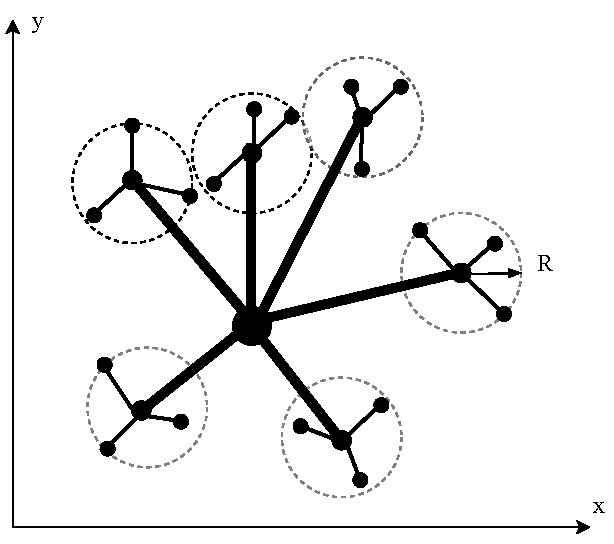
\includegraphics[pages=-]{./inc/img/bee.pdf}
	\caption{Схематичное изображение стратегии разведки двумерного пространства (жирные линии --- вылеты разведчиков, тонкие линии --- уточнение решений рабочими пчелами)}  
	\label{fig:bee}
\end{center}
\end{figure}  


\subsection{Описание алгоритма}

Рассмотрим задачу глобальной условной максимизации в гиперпараллелепипеде \textit{П}. Среди пчел $S = \{s_i, i \in [1:|S|]\}$ выделяем $|S^{\circ}| < |S|$ пчел-разведчиков. Для простоты записи будем считать, что эти пчелы являются первыми в рое $S$: 
$$S^{\circ} = \{s_i^{\circ}, i \in [1:|S^{\circ}|]\}.$$

Остальные пчелы роя 
$$S^w = \{s_i^w, i \in [1:|S^w|]\} = \{s_i, i \in [|S^{\circ}| + 1:|S|]\}$$ является рабочими пчелами; $|S^w| = |S| - |S^0|$. 

Значения фитнес-функции $f(x)$, cоответствующие текущему положению пчел $s_i^{\circ}$, $s_i^w$, обозначим $f(x_i^{\circ}) = f_i^{\circ}$, $f(x_i^w) = f_i^w$.

Множество \textit{элитных} участков обозначим $A^b = \{a_j^b, j \in [1:|A^b|]\}$. Множество перспективных участков обозначим $A^p = \{a_k^p, k \in [1:|A^p|]\}$. 

Пологаем, что участки $a_j^b$, $a_k^p$ представляют собой гиперпараллелепипеды в пространстве $R^{|x|}$, грани которых параллельны координатным плоскостям, центры находятся в точках $x_j^b$, $x_k^p$ и длины сторон равны $2r_l^b$, $2r_l^p$ соответственно (рис. \ref{fig:bee2}). Здесь $r_l^b, r_l^p, l \in [1:|x|]$ --- радиусы участков по соответствующим измерениям пространства поиска.  


\begin{figure}[h!]
	\begin{center}
	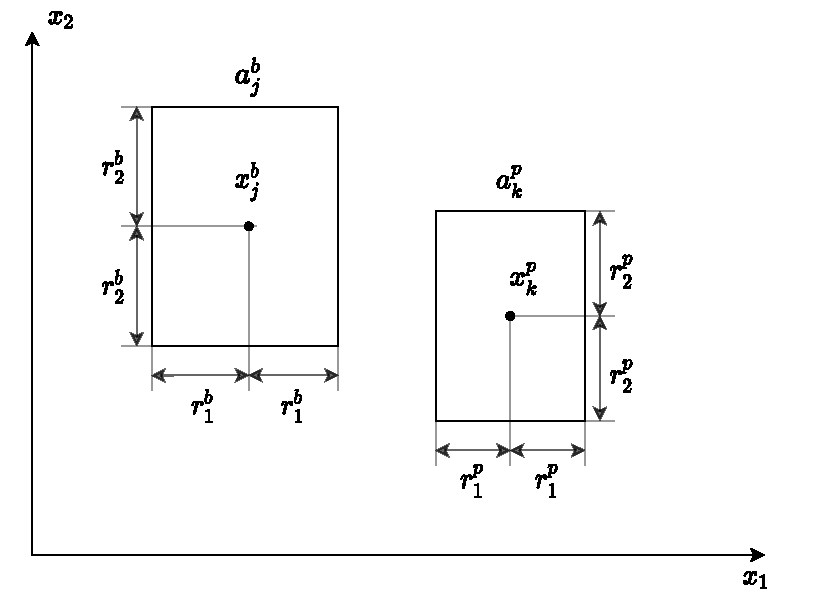
\includegraphics[pages=-]{./inc/img/bee2.pdf}
	\caption{К определению элитных и перспективных участков: $|x| = 2$}  
	\label{fig:bee2}
\end{center}
\end{figure}  


Во введенных обозначениях схема алгоритма имеет следующий вид.

\begin{enumerate}
	\item Генерируем случайные точки $x_i, i \in [1:|S^0|]$, равномерно распределенные во множестве \textit{П}, и отправляем в эти точки $|S^{\circ}|$, пчел-разведчиков $s_i^{\circ}$. Вычисляем в точках $x_i$ значения фитнес-функции $f_i^{\circ}$, сортируем величины $f_i^{\circ}$ по убыванию и представляем в виде линейного списка;
	\item Точки $x_j$, соответствующие первым $|A^b|$ элементам списка, объявляем центрами $x_j^b$ элитных участков $a_j^b, j \in [1:|A^b|]$. Аналогично точки $x_k, k \in [1:|A^p|]$, соответствующие последующим $|A^p|$ элементам списка, объявляем центрами перспективных участков $a_k^p$;
	\item В каждый из $a_j^b$ элитных и $a_k^p$ перспективных участков посылаем соответственно по $n_b$ и $n_p$ рабочих пчел $s_i^w \in S^w$, так что $$n_b |A^b| + n_p |A^p| = |S^w|.$$  Координаты точек, в которые посылаются эти пчелы, полагаем случайными величинами, равномерно распределенными в соответствующих гиперпараллелепипедах $a_j^b, a_k^p$. Во всех точках, в которые посланы пчелы вычисляем значения фитнес-функции;
	\item Проверяем выполнение условия окончания итераций. Если это условие выполнено, то в качестве решения задачи принимаем точку, соответствующую максимальному достигнутому значению фитнес-функции, и завершаем вычисления. В противном случае, приспособленности всех точек, найденных пчелами-разведчиками и рабочими пчелами, сортируем по убыванию и представляем в виде линейного списка. Переходим к шагу 2 \cite{karpenko} \cite{yang2}.
\end{enumerate}

В качестве условия окончания итераций может быть использовано достижение заданного числа итераций $t$ или стагнация вычислительного процесса в течение $\delta_t$ итераций.

\section{Муравьиный алгоритм} 
\subsection{Поведение муравьев в природе}
Муравьиные алгоритмы основаны на следующей особенности поведения муравьев в природе. При поиске путей к источникам пищи муравьи помечают пройденный путь специальным веществом --- \textit{феромоном} \cite{jason}. Остальные муравьи, попадая на такой путь, с большой вероятностью начинают
двигаться по этому пути, эта вероятность тем больше, чем больше концентрация феромона. Таким образом, феромон играет роль положительной обратной связи в системе --- чем больше муравьев движется по помеченному
пути, тем больше он становится привлекательным для других муравьев. В
результате, через некоторое время большая часть муравьев будет передвигаться от муравейника до найденного источника пищи по одному и тому же
пути.
Отличительными особенностями такого способа коммуникации являются:
\begin{enumerate}
	\item Обмен информацией между муравьями является непрямым (безадресным), а производится путем изменения окружающей муравьев среды;
	\item Информация является локально распределенной, другие муравьи могут получить доступ к ней, только переместившись в конкретную точку. 
\end{enumerate}


Интересной особенностью поведения муравьев является то, что найденный ими путь, при некоторых условиях, иногда оказывается \textit{кратчайшим}
постепенно за счет случайных флуктуаций, один из путей получает небольшое преимущество, которое очень быстро приводит к тому, что все муравьи
переключаются на этот путь. Если повторять этот опыт несколько раз, то
путем, связывающим муравейник с источником пищи. Этот факт был подтвержден опытами с настоящими муравьями. Схема одного такого классического опыта показана на рисунке \ref{fig:ant}. На рисунке \ref{fig:ant}.а имеется два пути одинаковой длины от муравейника до источника пищи. На начальном этапе опыта муравьи двигаются по обоим возможным направлениям, но
оказывается, что в среднем каждый из двух таких путей (равной длины)
выбирается примерно в половине случаев \cite{gorbunov}. 


% \begin{figure}[h!]
% 	\begin{center}
% 	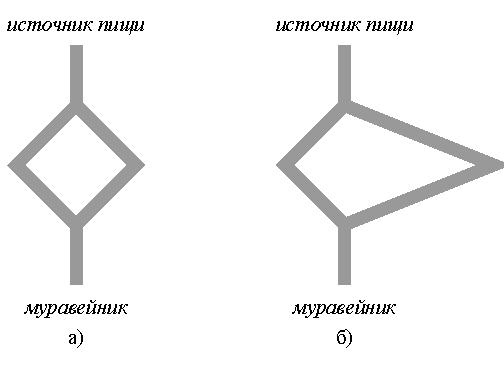
\includegraphics[pages=-]{./inc/img/ant.pdf}
% 	\caption{Схема опыта с двумя мостами}  
% 	\label{fig:ant}
% \end{center}

% % \begin{center}
% % 	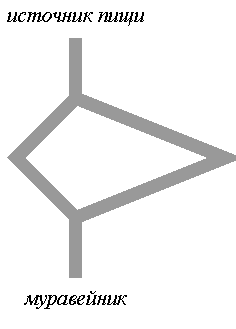
\includegraphics[pages=-]{./inc/img/ant2.pdf}
% % 	\caption{Схема опыта с двумя мостами}  
% % 	\label{fig:ant2}
% % \end{center}


% \end{figure}



\begin{figure}

\begin{minipage}{.49\textwidth}
	\centering
	
\includegraphics{inc/img/ant1.pdf} \\a)
  \end{minipage}
  \begin{minipage}{.49\textwidth}
	\centering
	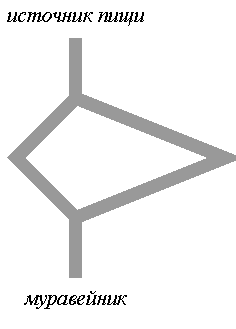
\includegraphics{inc/img/ant2.pdf} \\б)
  \end{minipage}
	\caption{Схема опыта с двумя мостами}  
	\label{fig:ant}
  
\end{figure}

% \begin{figure}[h!]
% 	\begin{minipage}[h][0.49\linewidth]
% 	
\includegraphics[ width=0.5\linewidth]{./inc/img/ant1.pdf}
% 	% \caption{Схема опыта с двумя мостами}  
% 	% \label{fig:ant}
% 	\end{minipage}

% \begin{minipage}[h][0.49\linewidth]
% 	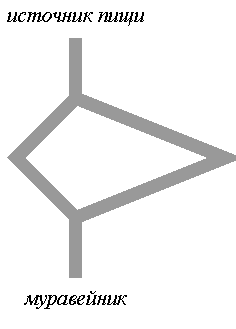
\includegraphics[width=0.5\linewidth]{./inc/img/ant2.pdf}
% 	% \caption{Схема опыта с двумя мостами}  
% 	% \label{fig:ant2}
% \end{minipage}
% \end{figure}


Иная ситуация наблюдается в том случае, если пути до пищи имеют
разную длину \ref{fig:ant}.б. Результатом такого опыта, как правило, является нахождение муравьями кратчайшего из двух путей. Этот результат
объясняется экспериментаторами тем, что короткие пути посещаются муравьями чаще, чем длинные, поэтому они и феромоном помечаются чаще,
что и приводит к усилению коротких путей по сравнению с длинными.


\subsection{Описание муравьиного алгоритма}

Описанная схема коммуникации муравьев легла в основу модели, разработанной Марко Дориго, и получившей название \textit{муравьиного алгоритма}. В этой модели предполагается, что средой обитания муравьев является
ненаправленный граф, в вершинах которого и располагаются муравьи. Все
ребра графа являются помеченными, в качестве метки ребра используется
действительное число, представляющее собой концентрацию феромона на
этом ребре.  

Перемещаются муравьи по ребрам графа. Муравей, находясь в вершине
$u$ графа, может переместиться на следующем шаге в вершину $v$ только в том
случае, если в графе имеется ребро $(u, v)$. Выбор ребра для перемещения
делается каждым муравьем на вероятностной основе, исходя из значений
концентрации феромона на ребрах исходящих из вершины $u$ --- чем больше концентрация (относительно других ребер), тем вероятнее выбор этого
ребра.  

При этом, на выбор ребра могут влиять и другие факторы, обычно опеределяемые спецификой решаемой задачи. Например, каждый муравей может иметь ограниченную память, в которой хранится номер последней посещенной им вершины. Тогда, ребро, ведущее в эту вершину (по которому был произведен последний переход) исключается из списка возможных
кандидатов на перемещение. Этот прием позволяет избежать короткого зацикливания муравья на одном ребре графа, но сохраняет возможность образования более длинных циклов\footnote{Известен природный аналог такого рода циклов --- так называемая «карусель смерти».}.  


Вероятность перехода из вершины $i$ в вершину $j$ определяется по формуле

$$	p_{i,j}={\frac {(\tau_{i,j}^{\alpha })(\eta_{i,j}^{\beta })}{\sum (\tau_{i,j}^{\alpha })(\eta_{i,j}^{\beta })}},$$

где $\eta_{i,j}$ --- расстояние от города $i$ до $j$, $\tau_{i,j}$ --- количество феромонов на ребре $ij$, $\alpha$ --- параметр влияния длины пути, $\beta$ --- параметр влияния феромона.

Уровень феромона обновляется в соответствии с формулой

$$	\tau_{i,j}=(1-\rho )\tau_{i,j}+\Delta \tau_{i,j},$$
где $\rho$ --- доля феромона, которая испарится, $\tau_{i,j}$ --- количество феромона на дуге $ij$, $\Delta \tau_{i,j}$ --- количество отложенного феромона, вычисляется по формуле

$$	\Delta \tau_{i,j}= \tau_{i,j}^0 + \tau_{i,j}^1 + ... + \tau_{i,j}^k,$$
где $k$ --- количество муравьев в вершине графа с индексами $i$ и $j$.

Описание поведения муравьев при выборе пути:
\begin{itemize}
\item муравьи имеют собственную «память».
	Поскольку каждый город может быть посещён только один раз, то у каждого муравья есть список уже посещенных городов --- список запретов.
	Обозначим через $J_{ik}$ список городов, которые необходимо посетить муравью $k$, находящемуся в городе $i$;
\item муравьи обладают «зрением» --- видимость есть эвристическое желание посетить город $j$, если муравей находится в городе $i$.
	Будем считать, что видимость обратно пропорциональна расстоянию между городами;
\item муравьи обладают «обонянием» --- они могут улавливать след феромона, подтверждающий желание посетить город $j$ из города $i$ на основании опыта других муравьёв.
	Количество феромона на ребре $(i,j)$ в момент времени $t$ обозначим через  $\tau_{i,j} (t)$;
\item пройдя ребро $(i,j)$, муравей откладывает на нём некоторое количество феромона, которое должно быть связано с оптимальностью сделанного выбора.
	Пусть $T _{k} (t)$ есть маршрут, пройденный муравьем $k$ к моменту времени $t$, $L _{k} (t)$ --- длина этого маршрута, а $Q$ --- параметр,
	имеющий значение порядка длины оптимального пути. Тогда откладываемое количество феромона может быть задано формулой
\end{itemize}

$$	{\displaystyle \Delta \tau_{i,j}^k={\begin{cases}Q/L_{k}, & {\mbox{если $k$-ый муравей прошел по ребру $ij$;}}\\0,&{\mbox{иначе.}}\end{cases}}}$$


На рисунке \ref{fig:class} приведена классификация ранее рассмотренных популяционных алгоритмов для задачи оптимизации поиска.\clearpage

\begin{figure}[h]
	\begin{center}
	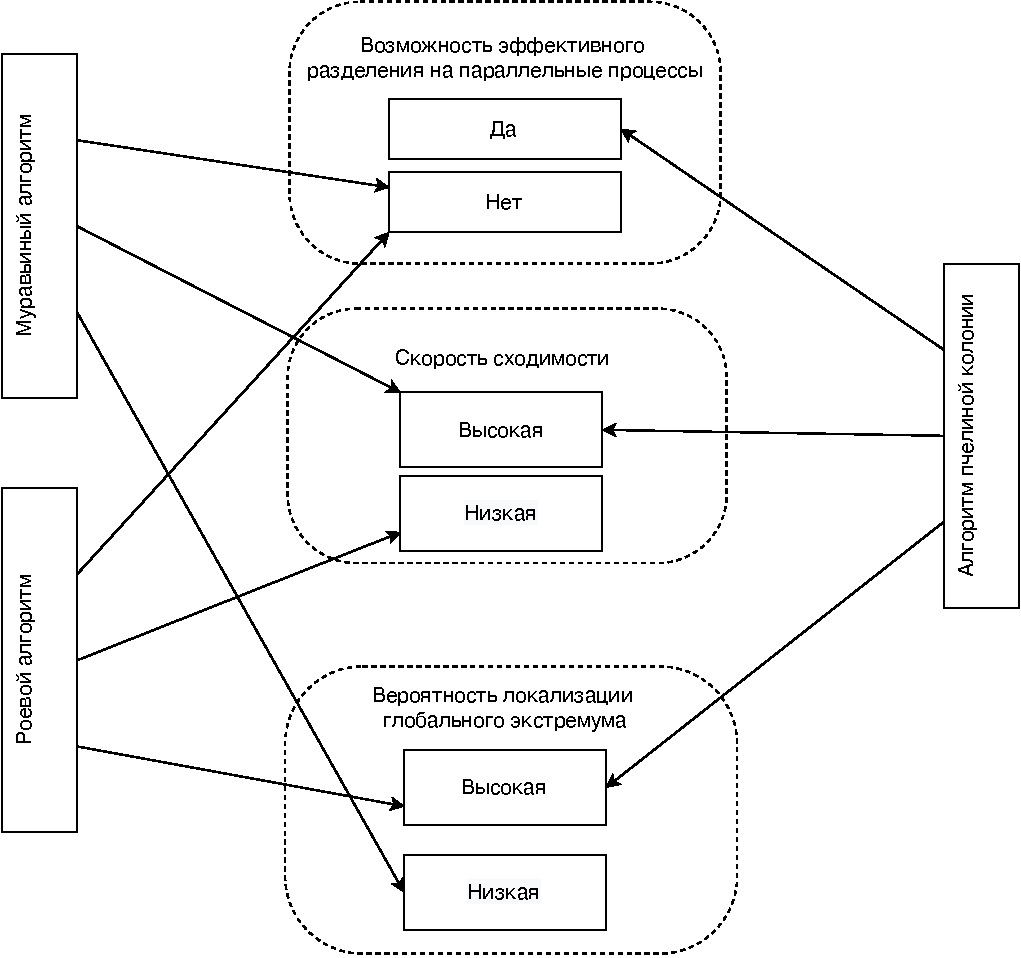
\includegraphics[pages=-, scale=0.95]{./inc/img/class.pdf}
	\caption{Классификация популяционных алгоритмов, вдохновленных живой природой}  
	\label{fig:class}
\end{center}
\end{figure}


